% =============================================
% 深度学习课程报告：三维重建与编辑
% 基于 xelatex/tectonic + ctex 编译
% =============================================
\documentclass[12pt, a4paper]{article}

\usepackage[fontset=none]{ctex}
\setCJKmainfont{Songti.ttc}[Path=/System/Library/Fonts/Supplemental/, FontIndex=3, BoldFont=Songti.ttc, BoldFeatures={FontIndex=3}]
\setCJKsansfont{STHeiti Light.ttc}[Path=/System/Library/Fonts/, BoldFont=STHeiti Light.ttc]
\setCJKmonofont{Songti.ttc}[Path=/System/Library/Fonts/Supplemental/, FontIndex=3, BoldFont=Songti.ttc, BoldFeatures={FontIndex=3}]
\setCJKfamilyfont{zhsong}{Songti.ttc}[Path=/System/Library/Fonts/Supplemental/, FontIndex=3, BoldFont=Songti.ttc, BoldFeatures={FontIndex=3}]
\setCJKfamilyfont{zhhei}{STHeiti Light.ttc}[Path=/System/Library/Fonts/, BoldFont=STHeiti Light.ttc]
\setCJKfamilyfont{zhfs}{Songti.ttc}[Path=/System/Library/Fonts/Supplemental/, FontIndex=3, BoldFont=Songti.ttc, BoldFeatures={FontIndex=3}]
\setCJKfamilyfont{zhkai}{Songti.ttc}[Path=/System/Library/Fonts/Supplemental/, FontIndex=3, BoldFont=Songti.ttc, BoldFeatures={FontIndex=3}]
\newcommand{\songti}{\CJKfamily{zhsong}}
\newcommand{\heiti}{\CJKfamily{zhhei}}
\newcommand{\fangsong}{\CJKfamily{zhfs}}
\newcommand{\kaishu}{\CJKfamily{zhkai}}

\usepackage[top=2.5cm, bottom=2.5cm, left=3cm, right=2.5cm]{geometry}
\usepackage{graphicx}
\usepackage{float}
\usepackage{subcaption}
\graphicspath{{figures/}}
\usepackage{booktabs}
\usepackage{tabularx}
\usepackage{multirow}
\usepackage{array}
\usepackage{amsmath, amssymb}
\usepackage{xcolor}
\usepackage{listings}
\usepackage{enumitem}
\usepackage{caption}
\captionsetup{font=small, labelfont=bf}
\usepackage[colorlinks=true, linkcolor=blue!70!black, urlcolor=blue, citecolor=green!50!black]{hyperref}
\usepackage{fancyhdr}

\newcommand{\courseName}{深度学习}
\newcommand{\expTitle}{课程报告}
\newcommand{\expFullTitle}{基于 VGGT 与 3DGS 的三维重建与编辑}
\newcommand{\academicYear}{2025-2026-2}
\newcommand{\college}{计算机学院}
\newcommand{\major}{计算机科学与技术}
\newcommand{\studentName}{胡鑫园等}
\newcommand{\studentID}{23050236}
\newcommand{\instructor}{任课教师}
\newcommand{\expDate}{2026 年 7 月 2 日}
\newcommand{\titleLogo}{hdu_title.png}

\pagestyle{fancy}
\fancyhf{}
\fancyhead[L]{\small \courseName}
\fancyhead[R]{\small \leftmark}
\fancyfoot[C]{\thepage}
\renewcommand{\headrulewidth}{0.4pt}

\lstset{
  basicstyle=\ttfamily\small,
  keywordstyle=\color{blue!70!black}\bfseries,
  commentstyle=\color{gray}\itshape,
  stringstyle=\color{red!70!black},
  numbers=left,
  numberstyle=\tiny\color{gray},
  numbersep=8pt,
  breaklines=true,
  frame=single,
  rulecolor=\color{black!30},
  backgroundcolor=\color{gray!5},
  showstringspaces=false,
  tabsize=4
}

\begin{document}

\begin{titlepage}
  \thispagestyle{empty}
  \centering
  \vspace*{2.0cm}
  \includegraphics[width=11cm]{\titleLogo}
  \vspace{2.2cm}

  {\fontsize{38}{50}\selectfont\heiti\bfseries \expTitle\par}
  \vspace{0.9cm}
  {\Large\bfseries （\academicYear）\par}
  \vspace{2.6cm}

  \newcommand{\infobox}[1]{\underline{\makebox[8.6cm][c]{\large #1}}}
  \renewcommand{\arraystretch}{1.75}
  \begin{tabular}{>{\large\bfseries}p{2.6cm} l}
    题\quad 目 & \infobox{\expFullTitle} \\
    学\quad 院 & \infobox{\college} \\
    专\quad 业 & \infobox{\major} \\
    学\quad 号 & \infobox{\studentID} \\
    学生姓名   & \infobox{\studentName} \\
    任课教师   & \infobox{\instructor} \\
    完成日期   & \infobox{\expDate} \\
  \end{tabular}
\end{titlepage}

\tableofcontents
\newpage

\section{实验目的}

本课程报告围绕“三维重建与三维编辑”这一深度学习应用任务展开。实验的核心目标不是单纯复现某一个模型，而是构建一条从真实校园图像采集到三维场景重建，再到语义级局部编辑的完整技术链路。具体目标如下：

\begin{itemize}
  \item 理解多视角三维重建、神经辐射场、3D Gaussian Splatting（3DGS）和前馈式几何估计模型 VGGT 的基本原理，分析它们在场景级重建中的互补关系。
  \item 以杭州电子科技大学校门、计算机学院、教室和实验室等真实场景为对象，完成图像或视频帧采集、相机几何估计、点云/高斯初始化、3DGS 优化和新视角渲染。
  \item 在重建场景上引入三维编辑思想，探索通过语义分割、多视角 grounding 和高斯显式参数操作实现删除、替换、插入和外观修改。
  \item 总结“高质量重建 + 显式高斯表示 + 语言驱动编辑”的优势、局限和可拓展方向，为后续校园数字孪生、AR 展示和低门槛三维内容创作提供技术参考。
\end{itemize}

\section{实验背景与原理}

\subsection{从图像到三维场景}

三维重建的目标是从一组二维观测中恢复场景的几何结构和外观表示。传统摄影测量和 Structure-from-Motion（SfM）方法首先通过特征匹配估计相机位姿，再三角化得到稀疏点云；Multi-View Stereo（MVS）进一步恢复稠密深度。该路线几何解释性强，但面对弱纹理、反光、遮挡和大范围光照变化时，结果容易出现空洞或漂移。

深度学习推动了三维表示从离散几何走向可微渲染。NeRF 将场景表示为连续的颜色-密度场，通过体渲染监督新视角合成，显著提升了复杂场景的照片级重建质量。然而，NeRF 依赖隐式网络查询，训练和渲染成本较高，且局部编辑不够直接。3D Gaussian Splatting 进一步使用大量带有位置、协方差、颜色和透明度的三维高斯作为显式场景单元，通过可微光栅化实现高质量实时渲染。对本实验而言，3DGS 的关键价值在于：每个高斯既是渲染单元，也是可选择、可移动、可删除和可重新优化的编辑单元。

从课程项目角度看，本任务同时涉及三类深度学习能力。第一是\textbf{几何感知能力}，即模型需要从多张二维图像中推断相机运动、深度和三维点；第二是\textbf{可微渲染优化能力}，即通过图像重建误差反向更新三维表示；第三是\textbf{多模态交互能力}，即把自然语言、二维视觉区域和三维对象对应起来。VGGT、3DGS 和三维编辑方法分别对应这三类能力，因此它们组合后比单独使用某一个模型更适合构建完整系统。

\subsection{VGGT 的前馈式几何估计}

VGGT（Visual Geometry Grounded Transformer）面向“从图像集合直接预测三维属性”的任务，将多张输入图像编码到统一 Transformer 表示中，并同时预测相机参数、深度图、点图和点跟踪。与传统 SfM 需要局部特征匹配、RANSAC 和 bundle adjustment 的多阶段流程不同，VGGT 更接近一个前馈式几何基础模型：它把多视角关系编码为网络推理问题，在稀疏视角、纹理不足或拍摄轨迹不规则时可为后续 3DGS 提供更稳定的相机与几何初始化。

在本实验流程中，VGGT 不替代 3DGS 的高保真外观优化，而是作为前端几何模块：输入校园场景的多视角图片后，先得到相机位姿、粗深度和初始点云，再将其转化为高斯初始化。这样可以减少纯 SfM 在校园场景中因玻璃、白墙、重复纹理和动态行人造成的失败风险。

\begin{figure}[H]
  \centering
  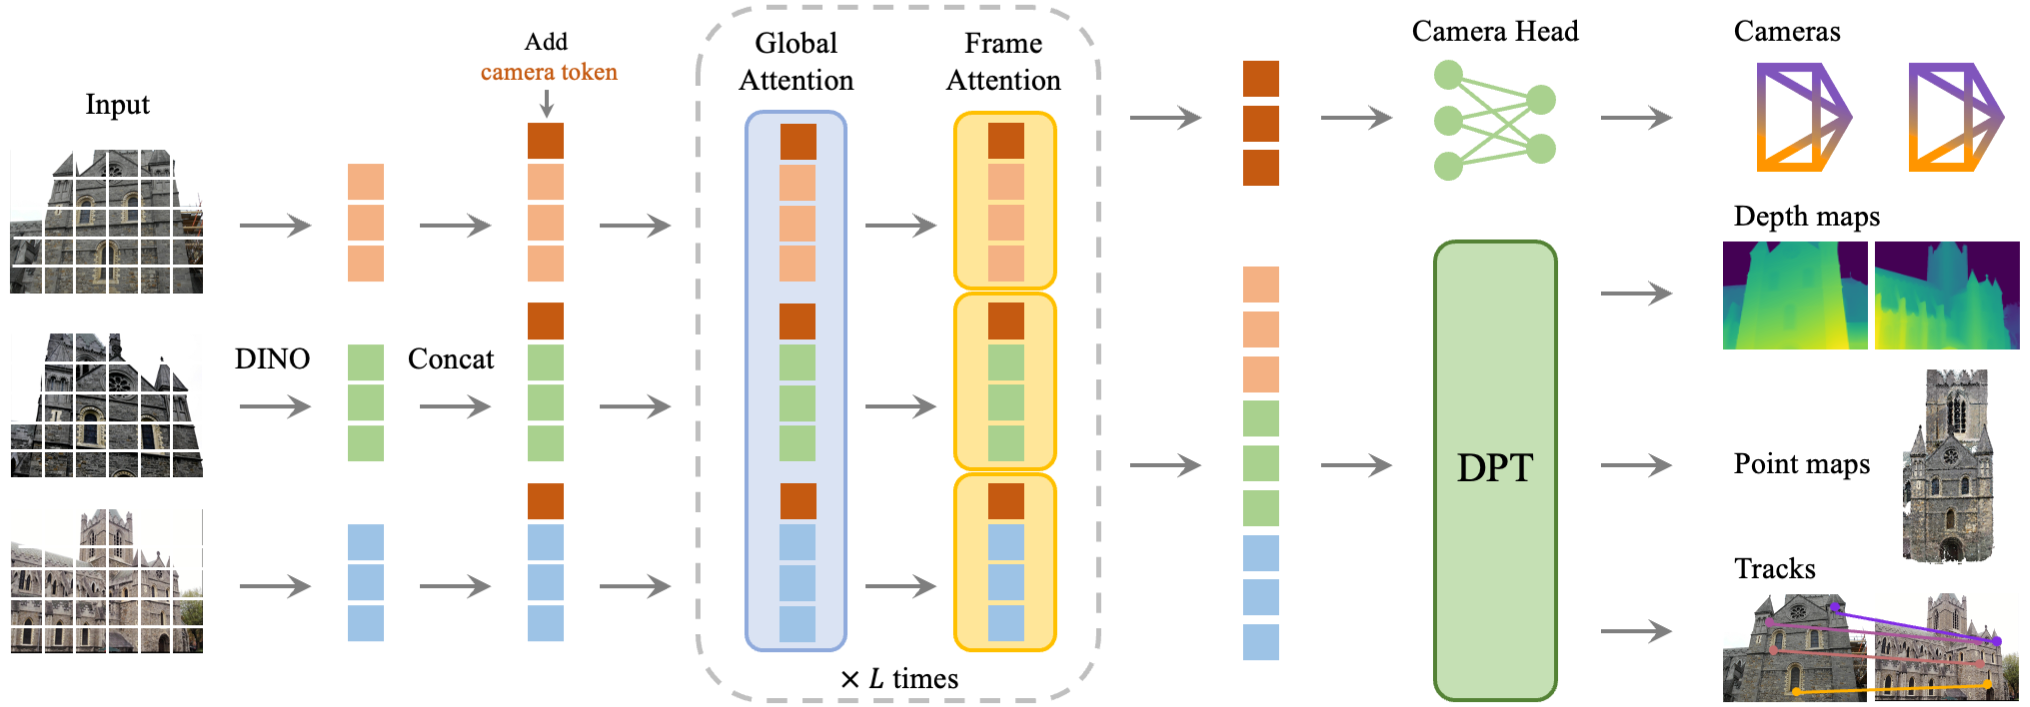
\includegraphics[width=0.95\linewidth]{vggt_architecture.png}
  \caption{VGGT 的整体架构示意图：多视角图像经 Transformer 统一编码后，同时输出相机、深度、点图和跟踪等几何结果。}
  \label{fig:vggt-architecture}
\end{figure}

VGGT 的优势在于把“相机估计”和“稠密几何预测”放入同一个前馈网络中建模。对于本实验的校园数据，这一点尤其重要：室外建筑通常存在重复窗格和大面积天空，室内实验室又有显示器反光、白墙和黑色桌面等低纹理区域，传统特征匹配很容易出现误匹配或匹配不足。VGGT 可以利用图像级上下文和跨视角注意力补足局部特征的不足，使重建前端不再完全依赖 SIFT/ORB 等手工特征。

\subsection{3D Gaussian Splatting 表示}

3DGS 将场景表示为高斯集合 $\mathcal{G}=\{g_i\}_{i=1}^{N}$。每个高斯通常包含中心位置 $\mu_i\in\mathbb{R}^{3}$、协方差矩阵 $\Sigma_i$、不透明度 $\alpha_i$ 和视角相关颜色 $c_i$。协方差常由旋转 $R_i$ 与尺度 $S_i$ 参数化：
\begin{equation}
  \Sigma_i = R_i S_i S_i^\top R_i^\top .
\end{equation}
渲染时，三维高斯被投影到图像平面形成二维椭圆 splat，并按深度顺序进行 alpha 合成。像素颜色可以写为：
\begin{equation}
  C(p)=\sum_{i\in \mathcal{N}(p)} T_i \alpha_i c_i,\quad
  T_i=\prod_{j<i}(1-\alpha_j),
\end{equation}
其中 $\mathcal{N}(p)$ 表示覆盖像素 $p$ 的高斯集合，$T_i$ 表示前方高斯的透射率。训练过程通过最小化渲染图像与真实图像之间的重建误差，联合优化高斯的位置、形状、透明度和颜色：
\begin{equation}
  \mathcal{L}_{rec}=(1-\lambda)\lVert I-\hat I\rVert_1+
  \lambda\,\mathcal{L}_{D\text{-}SSIM}(I,\hat I).
\end{equation}
这种表示兼顾了显式几何、可微优化和实时渲染，因此适合作为本报告中“重建-编辑”统一管线的核心表示。

\begin{figure}[H]
  \centering
  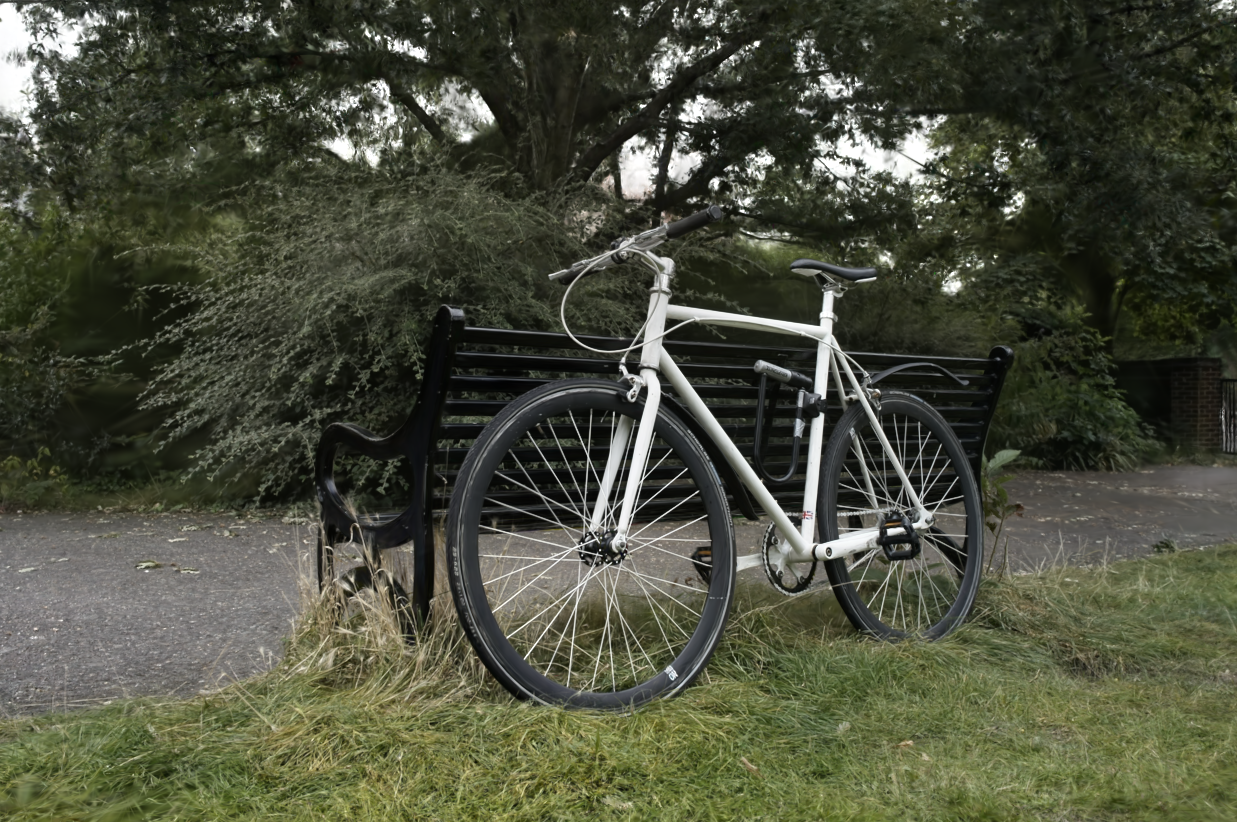
\includegraphics[width=0.92\linewidth]{official_3dgs_result.png}
  \caption{3DGS 官方项目展示的高质量新视角渲染效果。该类结果说明显式高斯表示可以在保持视觉质量的同时实现实时渲染。}
  \label{fig:official-3dgs}
\end{figure}

3DGS 的训练通常包含三类关键操作。第一是\textbf{初始化}：由 SfM 点云或 VGGT 点图生成初始高斯，每个点被赋予位置、颜色、尺度和不透明度。第二是\textbf{可微渲染}：将高斯投影到目标视角，用 alpha blending 形成渲染图，并通过图像损失反向传播。第三是\textbf{自适应密度控制}：对误差大的区域增加高斯，对贡献小或透明度低的高斯进行剪枝。校园场景中的窗框、桌椅边缘和文字标识通常需要更多高斯表达，而天空、白墙和远处树木则更依赖合理的剪枝与正则化。

\subsection{三维编辑的基本思想}

三维编辑的难点在于：用户指令通常是语义化的，例如“把桌边的椅子移走”或“在校门旁边插入一个导览牌”，而 3DGS 内部只是大量无序高斯参数。为连接自然语言与高斯集合，需要完成三步映射：
\begin{enumerate}[label=\arabic*.]
  \item 从多个代表视角渲染二维图像，并利用多模态大模型、检测模型或分割模型理解目标对象。
  \item 将二维 mask 或框通过可见性、深度和特征渲染反投到三维高斯集合，得到目标高斯子集 $\mathcal{G}_{target}$。
  \item 对目标高斯执行删除、复制、位姿变换、颜色调整、资产替换或局部重新优化，并保持未编辑区域 $\mathcal{G}_{keep}$ 的外观稳定。
\end{enumerate}
该思路与 LiSee 项目文档中“图文双驱的可编辑高精度三维资产生成系统”一致：真实照片负责提供可信场景基底，文本或图像生成负责补充新资产，语言推理式编辑负责降低用户操作门槛。

\begin{figure}[H]
  \centering
  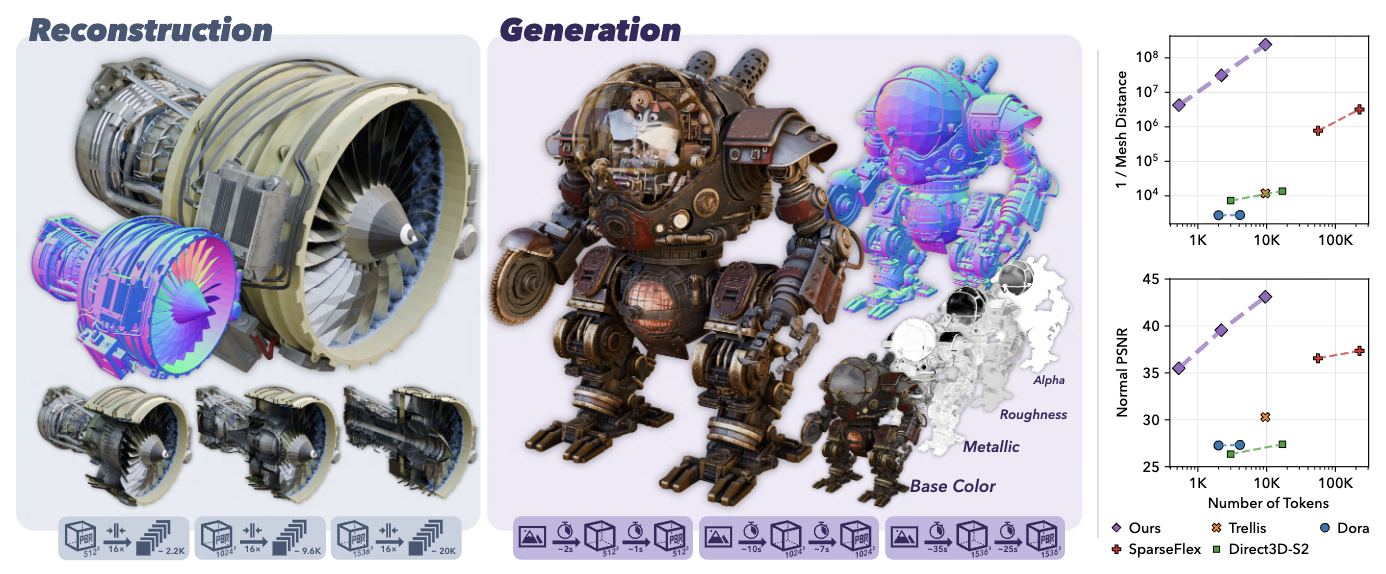
\includegraphics[width=0.95\linewidth]{lisee_reconstruction_generation.png}
  \caption{真实重建与生成式三维资产的互补关系：重建保证场景真实，生成提供可插入的新内容。}
  \label{fig:lisee-generation}
\end{figure}

进一步地，如果编辑操作要求“新增一个场景中原本不存在的物体”，仅靠 3DGS 参数编辑是不够的，还需要引入文本/图像到三维资产生成模型。Trellis 一类方法通过结构化三维 latent 将文本或图像条件解码为 3D Gaussians、网格等表示；LiSee 项目正是沿着这一思路，把真实重建、生成资产和语言编辑统一到一个可操作的三维空间中。

\begin{figure}[H]
  \centering
  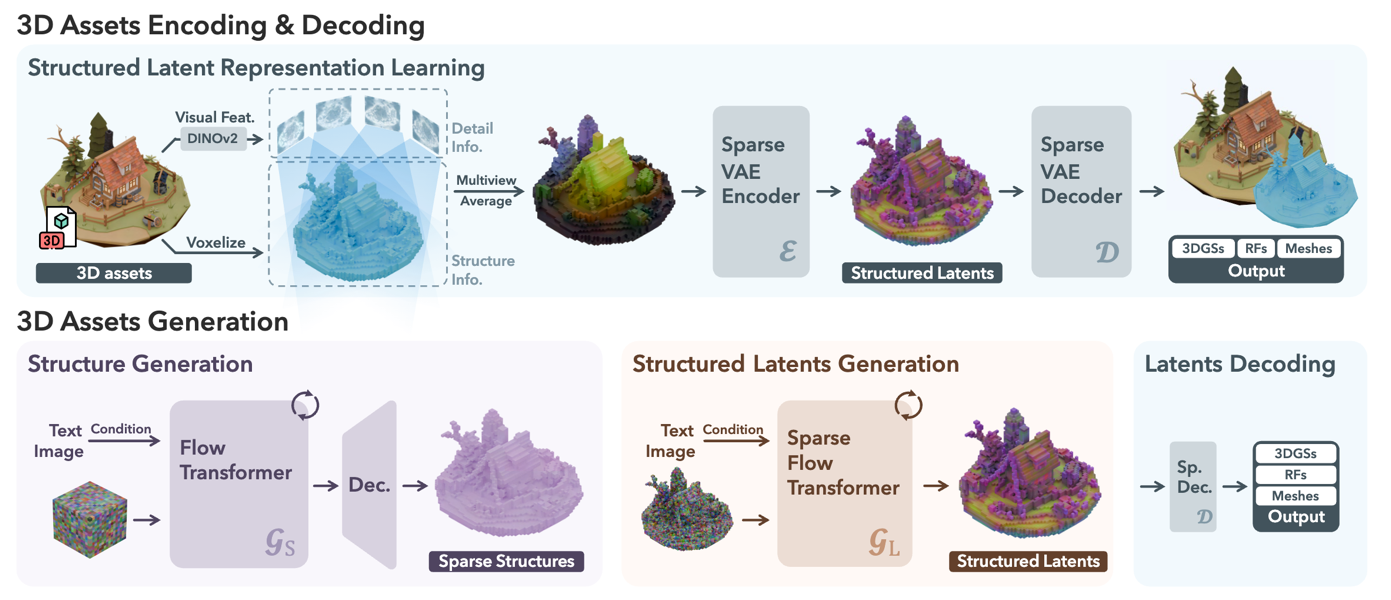
\includegraphics[width=0.95\linewidth]{trellis_pipeline.png}
  \caption{Trellis 类结构化三维 latent 生成流程，可为真实重建场景提供可插入、可转换格式的三维资产。}
  \label{fig:trellis-pipeline}
\end{figure}

\section{实验环境}

本实验以课程项目形式完成，重点验证算法流程和可视化效果。报告撰写与素材处理环境如下；模型训练和重建推理可根据 GPU 资源迁移到实验室服务器执行。

\begin{table}[H]
  \centering
  \caption{实验环境信息}
  \begin{tabularx}{\linewidth}{>{\centering\arraybackslash}p{3.5cm} >{\centering\arraybackslash}X}
    \toprule
    \textbf{项目} & \textbf{说明} \\
    \midrule
    操作系统 & macOS，本地完成报告、视频抽帧与 LaTeX 编译 \\
    深度学习框架 & PyTorch，可用于 VGGT、3DGS 及编辑模块推理 \\
    三维重建工具 & VGGT 前馈几何估计，3D Gaussian Splatting 优化与实时渲染 \\
    图像/视频处理 & FFmpeg 抽取校园场景视频关键帧，PNG 图片用于报告展示 \\
    硬件建议 & NVIDIA GPU（显存 12GB 及以上更适合 3DGS 优化和多视角渲染） \\
    \bottomrule
  \end{tabularx}
\end{table}

\section{实验设计}

\subsection{整体技术路线}

本实验采用“采集-几何估计-高斯重建-语义定位-局部编辑”的流水线。首先对校园场景进行环绕拍摄或短视频采集，并从视频中抽取覆盖不同视角的关键帧；随后使用 VGGT 估计相机位姿、深度和初始点云；再将点云初始化为 3DGS，通过可微渲染优化得到可实时浏览的三维场景；最后在场景中执行编辑操作，包括对象删除、局部替换、生成资产插入和外观调整。图 \ref{fig:vggt-3dgs-pipeline} 给出了本报告采用的重建主线，图 \ref{fig:pipeline} 则对应后续语言编辑模块。

\begin{figure}[H]
  \centering
  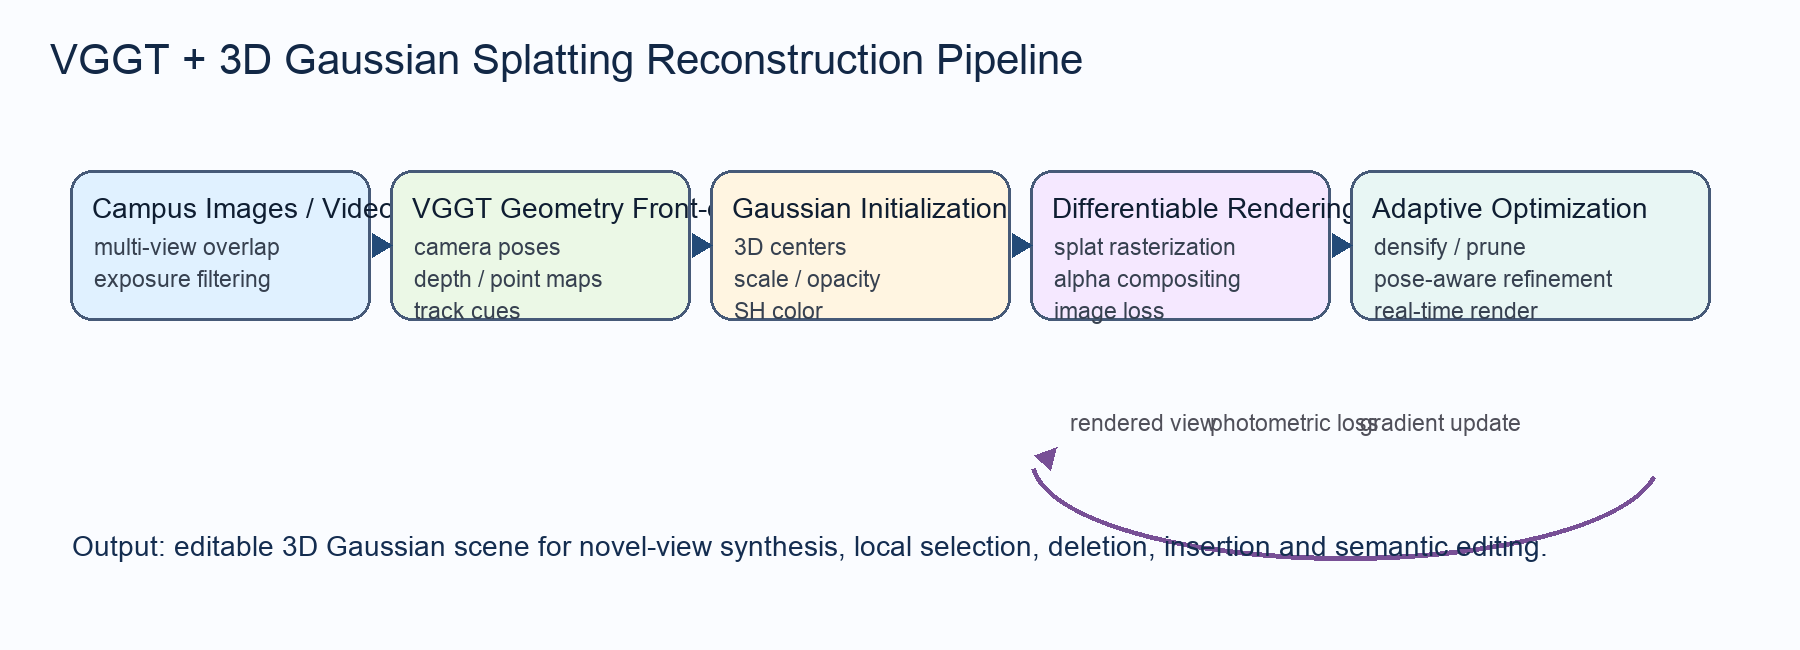
\includegraphics[width=0.98\linewidth]{vggt_3dgs_pipeline.png}
  \caption{本文采用的 VGGT + 3DGS 重建 pipeline：VGGT 负责前馈式几何估计，3DGS 负责显式高斯优化与实时渲染。}
  \label{fig:vggt-3dgs-pipeline}
\end{figure}

\begin{figure}[H]
  \centering
  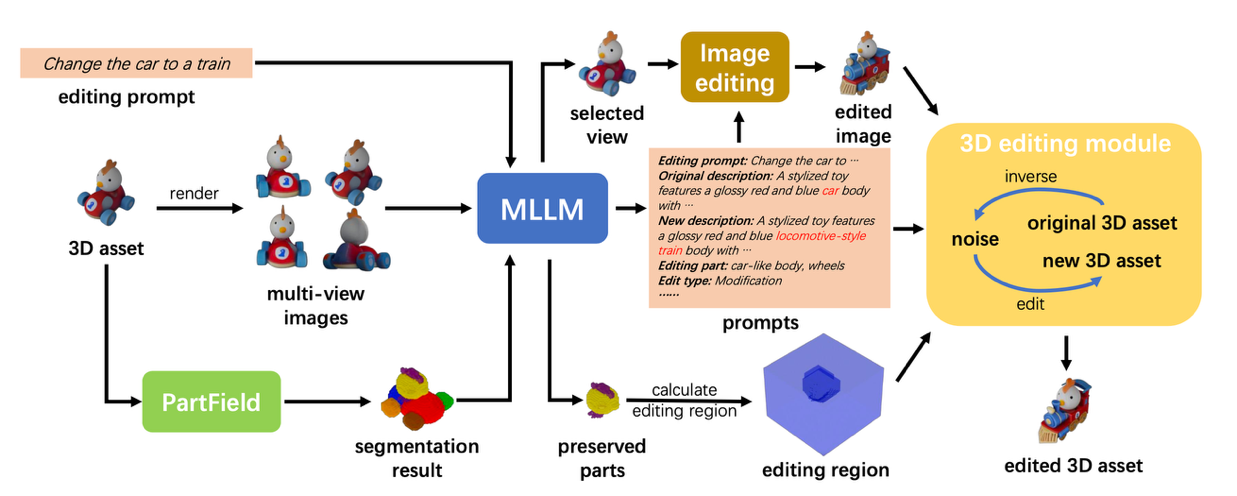
\includegraphics[width=0.92\linewidth]{realm_pipeline.png}
  \caption{语言驱动三维编辑的典型流程：多模态理解、目标区域定位、三维对象选择与编辑执行。}
  \label{fig:pipeline}
\end{figure}

该设计的核心是把 VGGT 和 3DGS 的职责拆开：VGGT 输出的是“可用于初始化的几何”，3DGS 输出的是“可用于渲染和编辑的场景表示”。如果直接用 VGGT 的点云做展示，细节纹理和新视角连续性不够；如果只用 3DGS 而没有可靠前端，在稀疏视角或弱纹理场景中容易初始化失败。因此二者结合可以在课程实验条件下获得更稳健的结果。

\subsection{校园数据采集}

数据采集覆盖了四类场景：校门等室外地标、计算机学院建筑、教室/实验室室内空间以及带有局部物体的展示场景。采集时尽量遵循三条原则：
\begin{itemize}
  \item 相邻视角保持 60\% 以上重叠，避免相机位姿估计断裂；
  \item 围绕主体形成弧形或闭环轨迹，覆盖正面、侧面和局部细节；
  \item 控制曝光变化和运动模糊，尽量避开大面积动态行人。
\end{itemize}

对于视频输入，本实验使用 FFmpeg 抽取关键帧。实际项目中可按固定间隔抽帧，也可根据清晰度、视差和图像重叠度筛选关键帧。示例命令如下：

\begin{lstlisting}[language=bash, caption={从校园重建视频中抽取代表视角}]
ffmpeg -ss 5 -i input_scene.mp4 -frames:v 1 figures/view_01.png
\end{lstlisting}

抽帧后需要进行两类筛选。第一类是\textbf{质量筛选}：剔除运动模糊、曝光突变、画面遮挡严重的帧；第二类是\textbf{几何筛选}：保证相邻帧既有足够重叠，又有一定视差。如果所有帧都来自几乎相同的视角，模型只能恢复平面化外观；如果相邻帧变化过大，匹配和跨视角推理又会变得困难。本实验最终保留校门、计算机学院、教室和实验室四组素材，用于覆盖室外大尺度、室内弱纹理、局部物体密集和视频录屏重建等不同情况。

\subsection{VGGT 与 3DGS 的衔接}

VGGT 输出的相机参数和三维点为 3DGS 初始化提供了几何先验。设 VGGT 对第 $k$ 张图像预测相机外参 $T_k=[R_k|t_k]$、内参 $K_k$ 和深度 $D_k$，则像素 $p=(u,v)$ 可反投影为：
\begin{equation}
  X_{k,p}=R_k^\top\left(D_k(p)K_k^{-1}[u,v,1]^\top-t_k\right).
\end{equation}
合并多视角点后，可通过体素下采样和可见性过滤得到初始化点云，再为每个点分配初始高斯尺度、颜色和不透明度。相较随机初始化或仅依赖稀疏 SfM 点，VGGT 初始化能够让 3DGS 更快进入稳定优化阶段，减少室内白墙、走廊重复纹理和弱纹理地面造成的漂浮高斯。

实际衔接时还需要处理坐标系和尺度问题。VGGT 输出的点图通常位于模型定义的相机/世界坐标中，而 3DGS 训练脚本往往遵循 COLMAP 风格的相机参数与点云格式。因此需要将内参、外参、点云颜色和图像文件组织为统一数据接口。对于校园场景，建议在进入 3DGS 之前增加三个检查：相机轨迹是否连续、点云尺度是否异常、点云是否覆盖主体区域。若这三项检查失败，即使后续优化损失下降，也可能只是过拟合少数视角，而不是形成真实三维结构。

\subsection{编辑模块设计}

编辑模块以 3DGS 的显式高斯为操作对象。对于删除或移动操作，系统只需定位目标高斯集合并改变其参数；对于替换或插入操作，则需要将外部生成资产对齐到真实场景中。设待插入资产的高斯集合为 $\mathcal{G}_{obj}$，真实场景为 $\mathcal{G}_{scene}$，相似变换为 $(s,R,t)$，则资产中每个高斯中心和协方差变换为：
\begin{equation}
  \mu'_i=sR\mu_i+t,\quad
  \Sigma'_i=s^2R\Sigma_iR^\top.
\end{equation}
完成初始插入后，只在接触边界和邻域区域做局部优化：
\begin{equation}
  \min_{\mathcal{G}_{local}} \mathcal{L}_{rec}
  +\lambda_b \mathcal{L}_{boundary}
  +\lambda_c \mathcal{L}_{color}
  +\lambda_r \mathcal{L}_{reg}.
\end{equation}
其中 $\mathcal{L}_{boundary}$ 用于缓解边界割裂，$\mathcal{L}_{color}$ 用于光照和色调一致化，$\mathcal{L}_{reg}$ 防止插入资产形状被过度破坏。

对于替换和插入类编辑，报告还参考 LiSee 项目中的“图文双驱”思路：当用户给出文字指令时，系统可以先生成或检索目标三维资产，再将资产转换为 3DGS 或 mesh/高斯混合表示，最后通过尺度归一化、底面估计和局部颜色校正放入真实场景。图 \ref{fig:trellis-examples} 展示了生成资产分支的典型结果，这类资产可作为校园场景中虚拟展板、装饰物、导览标识等新增内容的来源。

\begin{figure}[H]
  \centering
  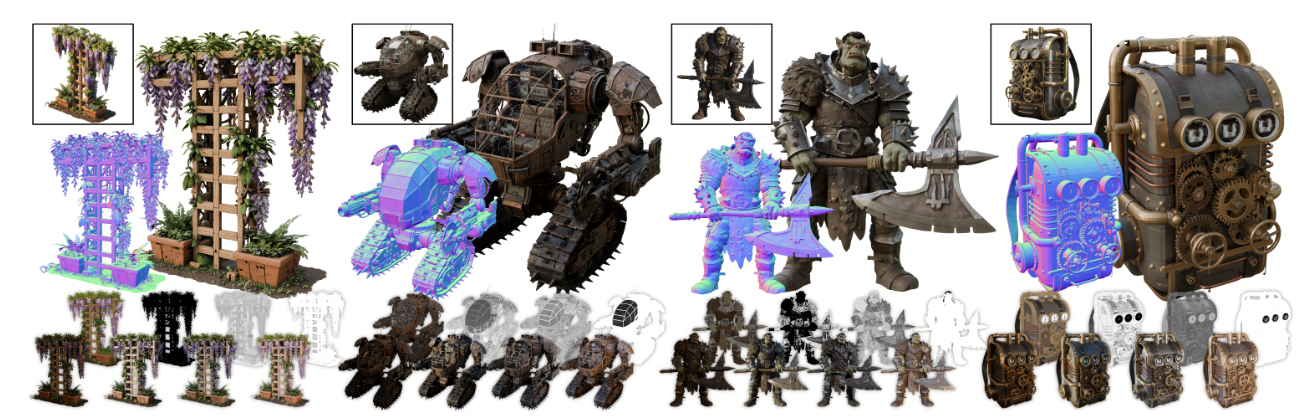
\includegraphics[width=0.95\linewidth]{trellis_generation_examples.png}
  \caption{文本/图像驱动的三维资产生成结果示例，可作为真实校园重建场景中的可插入对象。}
  \label{fig:trellis-examples}
\end{figure}

\section{实验过程与结果分析}

\subsection{校园场景重建结果}

图 \ref{fig:campus-scenes} 展示了本实验使用的校园场景素材与重建视角。校门和计算机学院场景体现了室外建筑结构的尺度感；教室和实验室场景包含桌椅、显示器、墙面和局部装饰，对几何连续性和细节纹理提出了更高要求。

\begin{figure}[H]
  \centering
  \begin{subfigure}{0.48\linewidth}
    \centering
    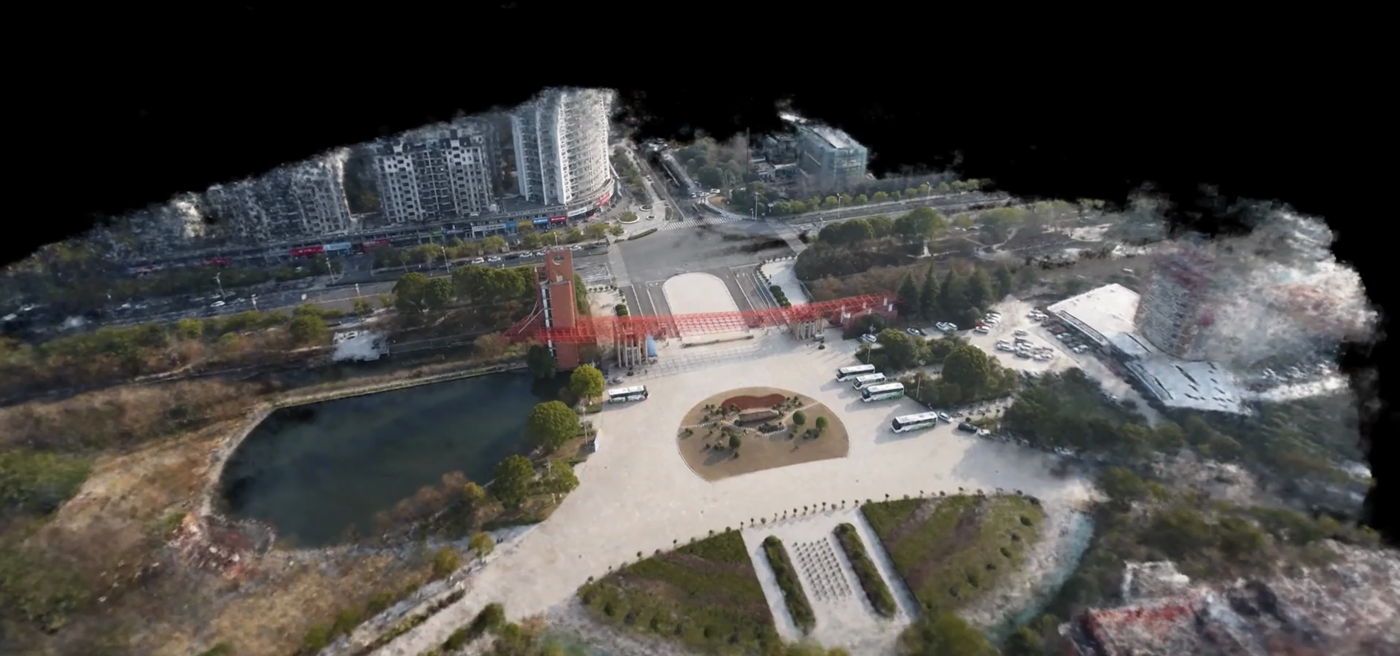
\includegraphics[width=\linewidth]{hdu_gate_view1.png}
    \caption{杭州电子科技大学校门}
  \end{subfigure}
  \hfill
  \begin{subfigure}{0.48\linewidth}
    \centering
    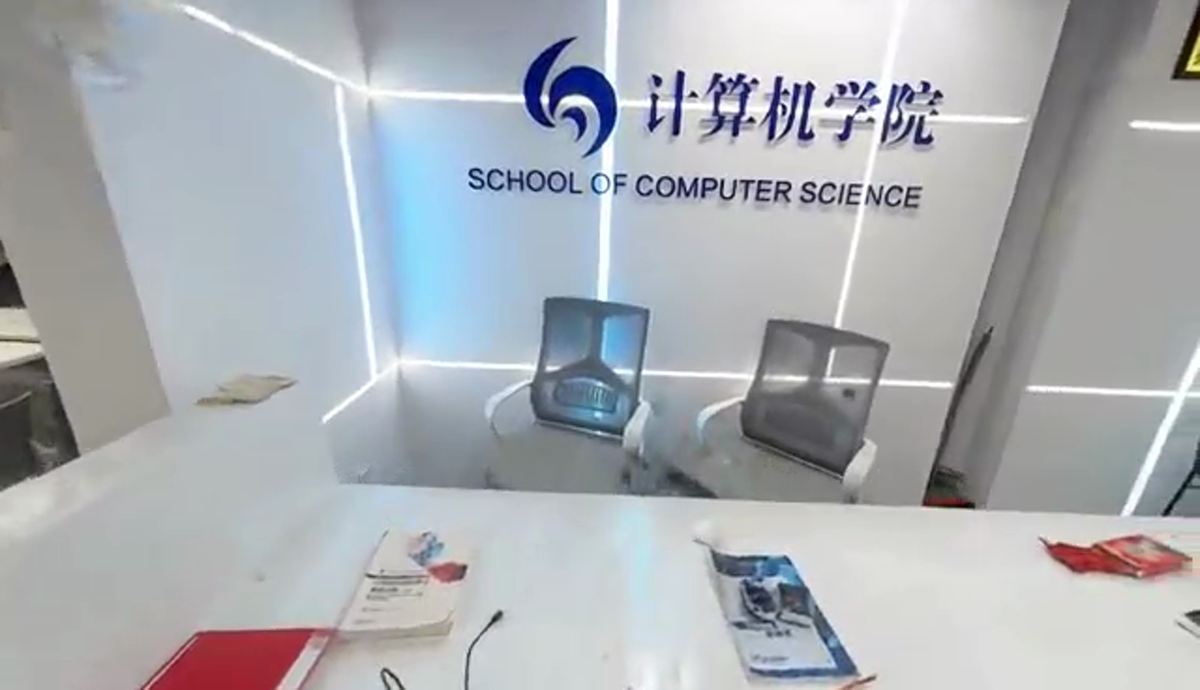
\includegraphics[width=\linewidth]{college_gs_view.png}
    \caption{计算机学院重建视角}
  \end{subfigure}

  \vspace{0.5em}
  \begin{subfigure}{0.48\linewidth}
    \centering
    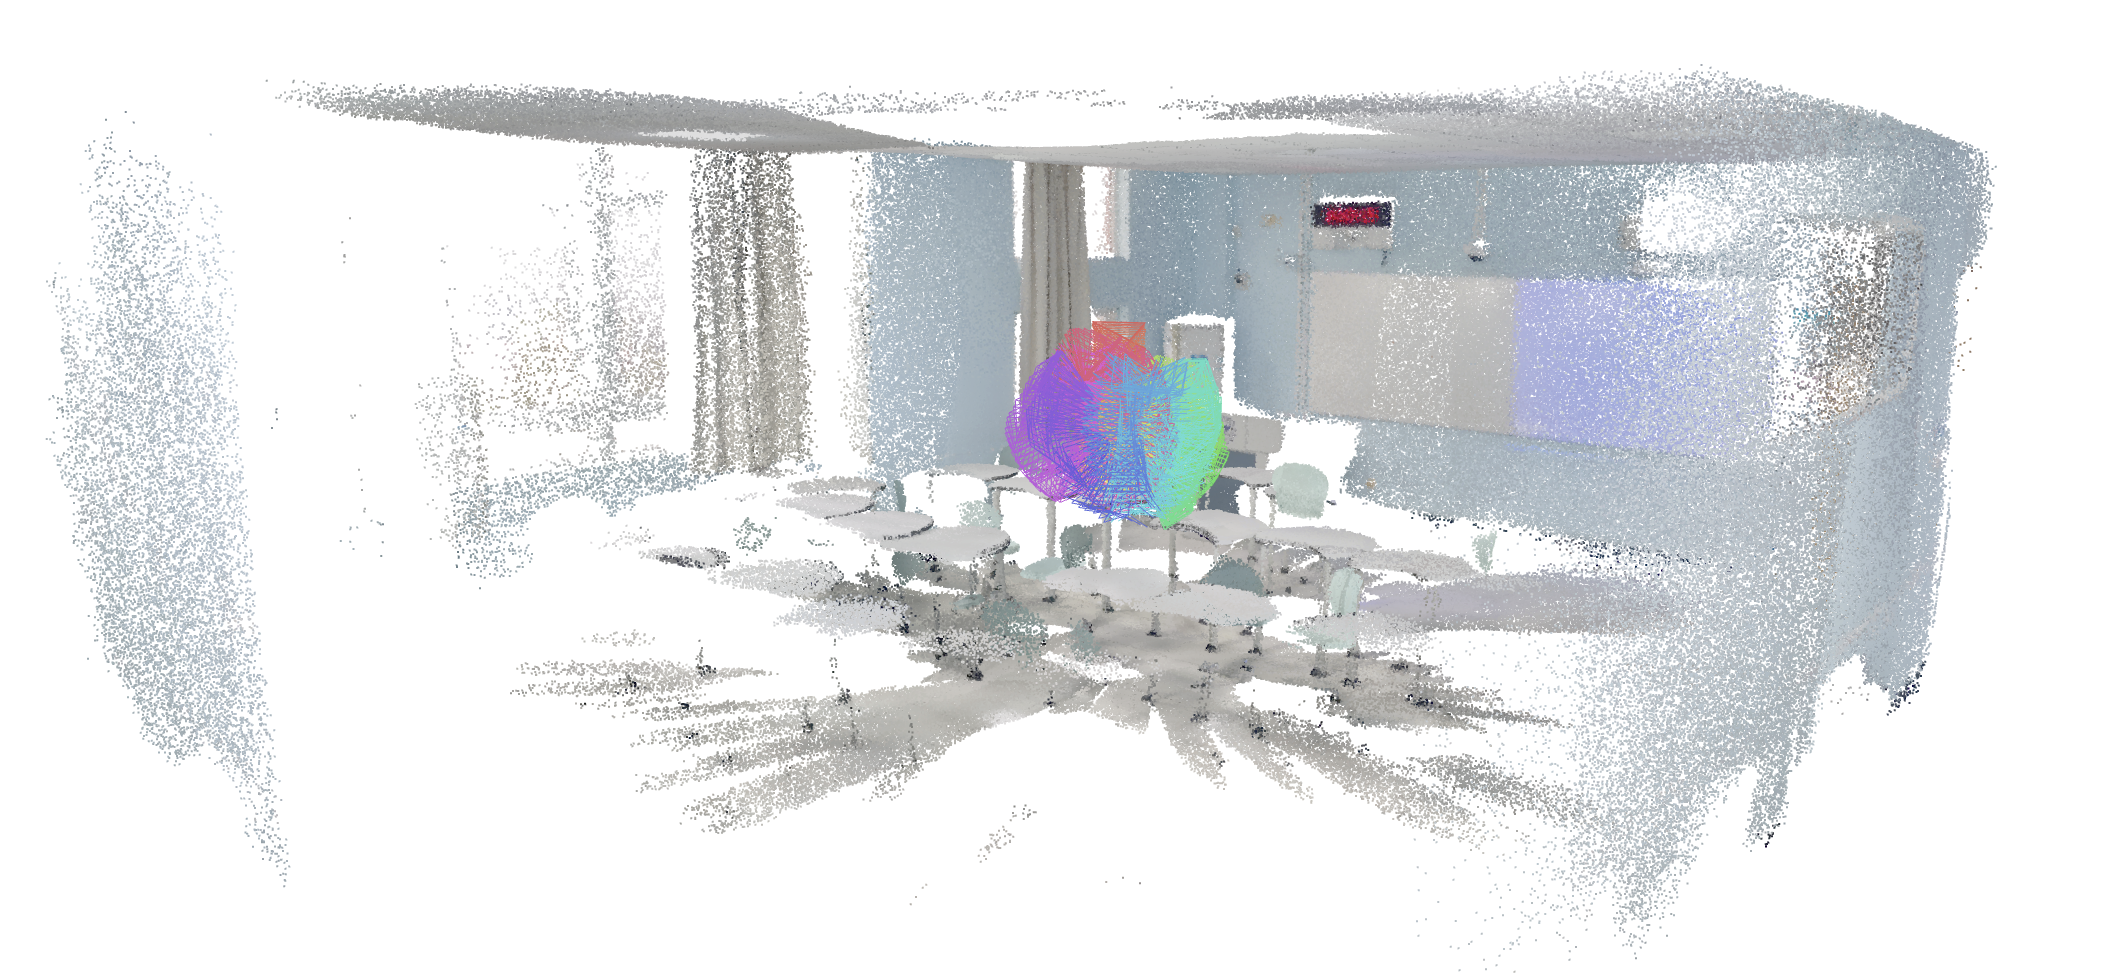
\includegraphics[width=\linewidth]{classroom.png}
    \caption{教室场景输入/结果}
  \end{subfigure}
  \hfill
  \begin{subfigure}{0.48\linewidth}
    \centering
    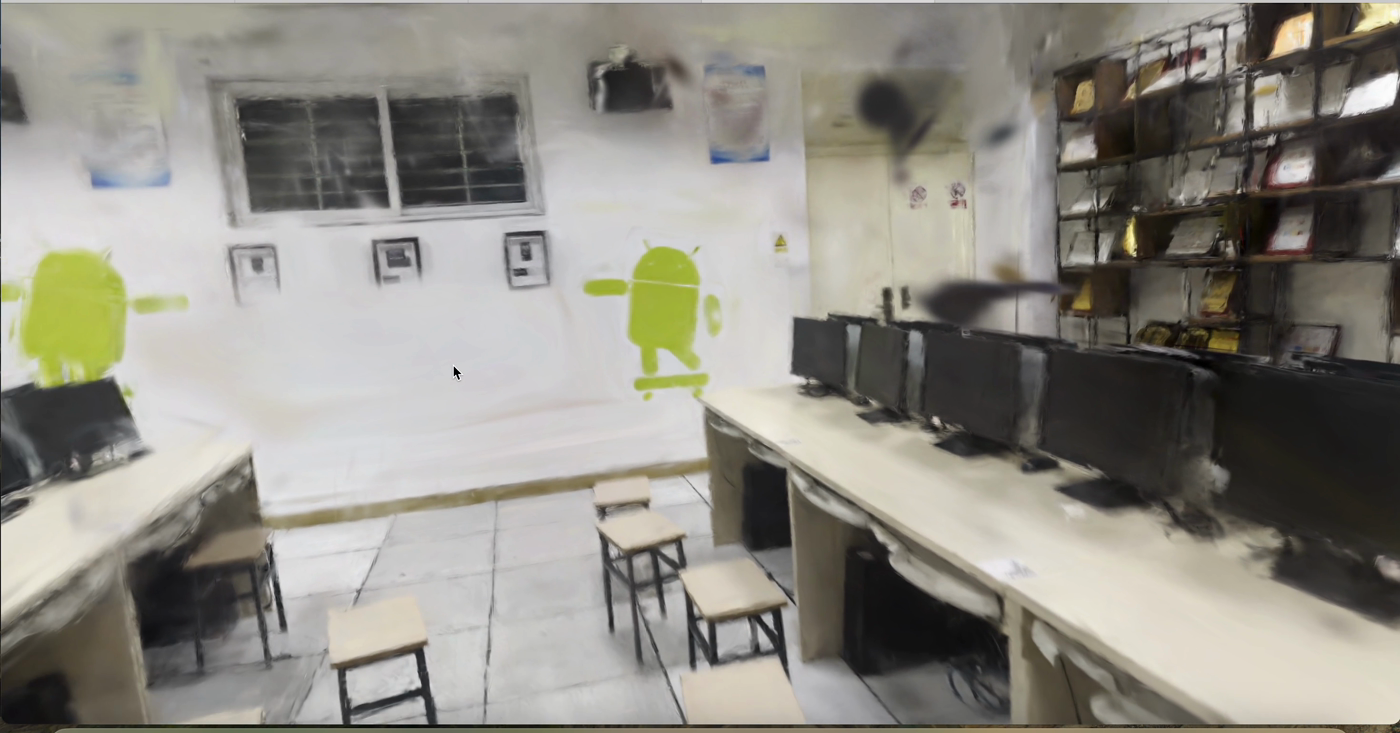
\includegraphics[width=\linewidth]{redpanda_3d_view.png}
    \caption{实验室场景局部渲染}
  \end{subfigure}
  \caption{校园多场景三维重建素材与代表视角。}
  \label{fig:campus-scenes}
\end{figure}

为了更直观地观察重建结果在不同视角下的一致性，本实验还从各段视频中抽取了多个视角帧，如图 \ref{fig:campus-multiview} 所示。多视角展示比单张截图更能暴露三维重建质量：如果模型只是记住某一个视角的纹理，换到侧面或远处视角时会出现明显拉伸；如果几何结构稳定，则主体边界、地面-墙面关系和物体相对位置应在多个视角中保持连续。

\begin{figure}[H]
  \centering
  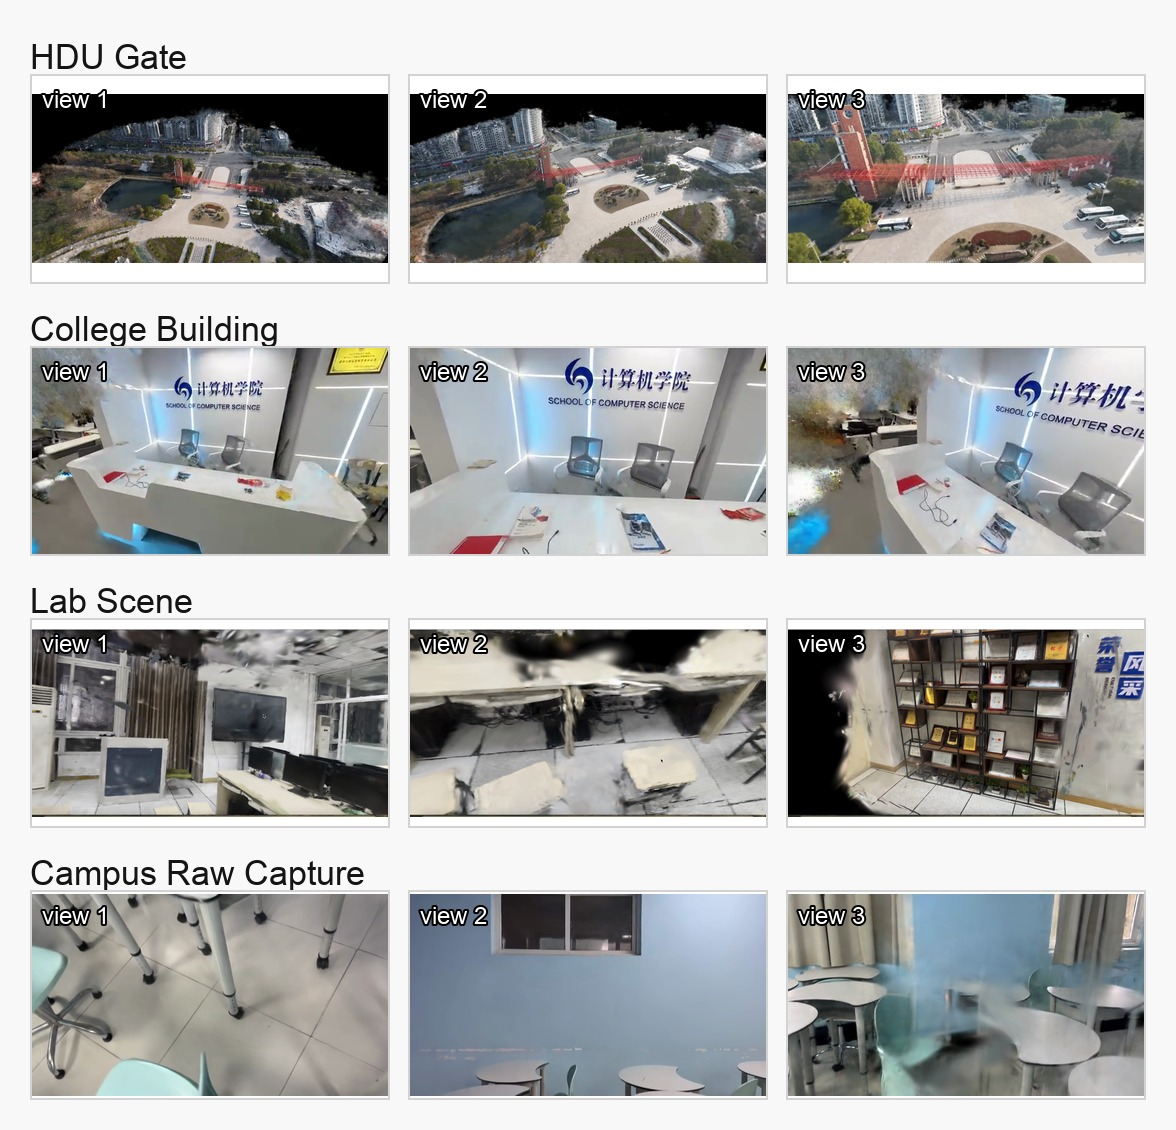
\includegraphics[width=0.98\linewidth]{campus_multiview_grid.jpg}
  \caption{校园场景多角度关键帧展示：校门、计算机学院、实验室和原始采集片段均覆盖不同观察方向。}
  \label{fig:campus-multiview}
\end{figure}

从结果可以观察到，3DGS 对建筑轮廓、桌面、显示器等具有明确边界的物体能形成较稳定的视觉表达；在墙面、天花板和远处低纹理区域，仍可能出现模糊或局部漂浮。这与 3DGS 的表示特性有关：高斯数量会优先分配给多视角一致且具有显著颜色梯度的位置，而弱纹理区域缺少足够监督信号。VGGT 提供的深度和相机先验可以缓解这一问题，但不能完全替代高质量采集。

室外校门场景的主要挑战是尺度大、背景远、天空和树木区域纹理不稳定。室内实验室场景则相反，尺度较小但局部物体密集，显示器、桌面、椅子和墙面装饰互相遮挡，容易在高斯优化时形成局部漂浮。计算机学院场景的视频分辨率较低，说明输入压缩会降低边缘细节；但建筑立面具有明显几何线条，仍有利于相机轨迹估计和高斯收敛。教室场景中重复桌椅较多，是检测多视角一致性的典型难例。

\subsection{重建质量分析}

本实验从视觉质量、几何稳定性和可编辑性三个维度评价重建结果。

\begin{table}[H]
  \centering
  \caption{不同校园场景的重建现象分析}
  \begin{tabularx}{\linewidth}{p{2.8cm} p{3.2cm} X}
    \toprule
    \textbf{场景} & \textbf{主要优势} & \textbf{主要问题与原因} \\
    \midrule
    校门室外场景 & 建筑轮廓清晰，主体尺度稳定 & 天空、远处树木和反光区域容易被模糊化，动态物体会带来不一致观测 \\
    计算机学院 & 立面结构和道路关系较明确 & 远距离纹理细节有限，视频压缩会影响边缘质量 \\
    教室 & 桌椅、讲台等物体结构较丰富 & 重复桌椅导致局部匹配混淆，白墙区域几何约束弱 \\
    实验室 & 显示器、桌面和装饰物便于局部编辑 & 录屏或快速移动视角带来模糊，黑色物体细节较难恢复 \\
    \bottomrule
  \end{tabularx}
\end{table}

课程实验中最关键的认识是：重建质量不只由模型决定，还强依赖采集策略。对于 3DGS，输入视角的覆盖度、曝光一致性和相机轨迹平滑程度会直接影响可优化性；对于 VGGT，图像集合中的重叠关系和场景静态性会影响前馈几何推理的稳定性。因此，后续若追求更高质量，应优先改进采集：慢速环绕、减少运动模糊、增加近景补拍，并对视频抽帧做清晰度筛选。

如果进一步量化评估，可采用 PSNR、SSIM 和 LPIPS 衡量新视角渲染质量，并使用相机轨迹连续性、点云覆盖率和目标区域重投影误差作为几何指标。对于课程报告，目前更强调流程验证和可视化分析，因此本文采用“代表视角 + 多视角一致性 + 场景问题诊断”的方式呈现实验结果。

\subsection{三维编辑实验设计与展示}

在完成重建后，编辑实验关注两个问题：第一，用户能否用自然语言或图像提示定位目标区域；第二，局部编辑后未选中区域能否保持稳定。图 \ref{fig:realm-overview} 展示了 REALM 类方法的场景级推理编辑思路，系统先通过多视角观察理解三维场景，再将二维语义结果聚合到三维高斯对象上。

\begin{figure}[H]
  \centering
  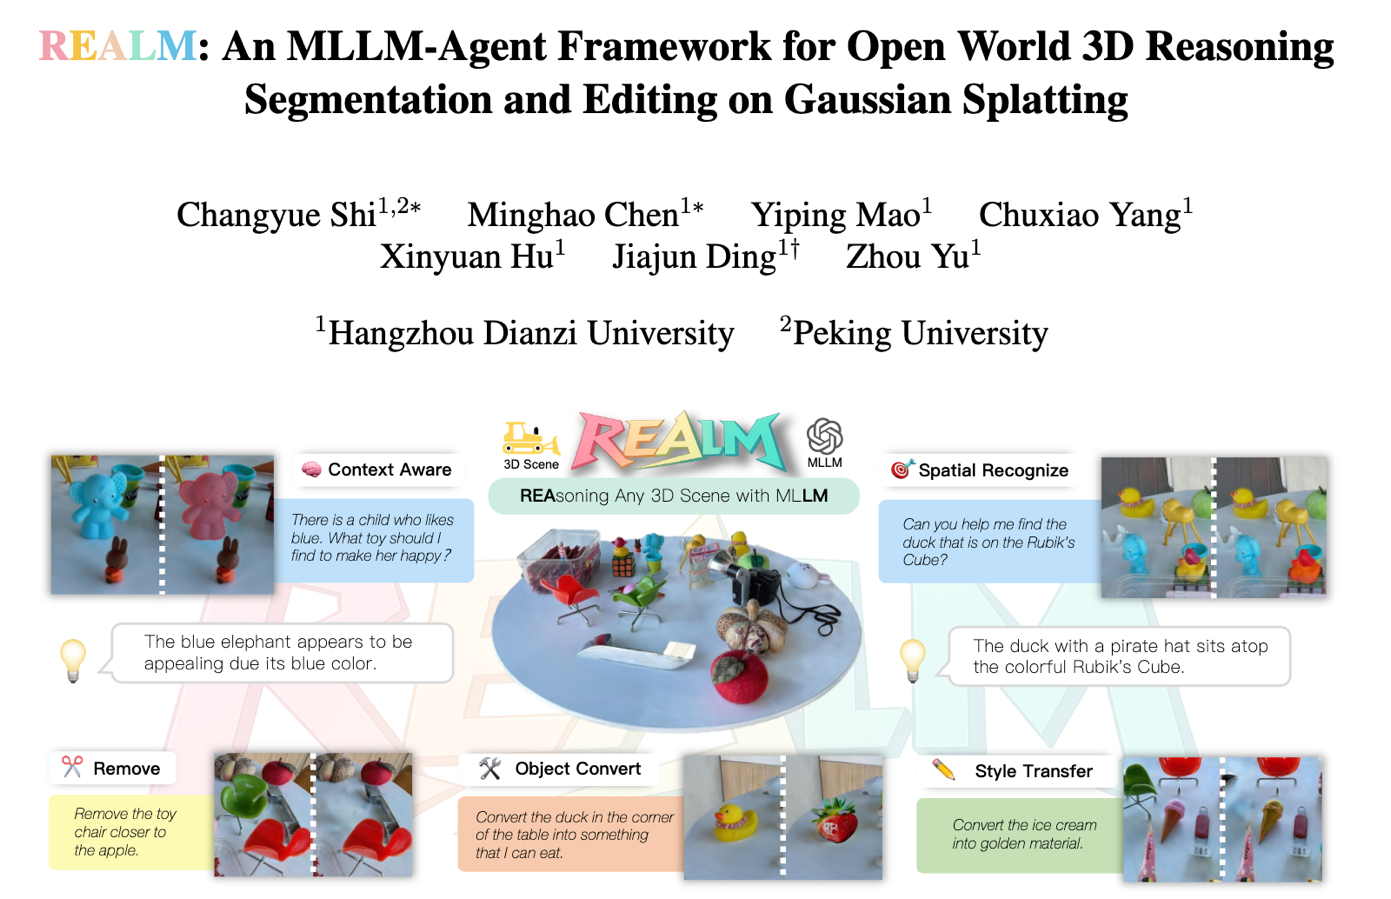
\includegraphics[width=0.95\linewidth]{realm_overview.png}
  \caption{基于 MLLM agent 的开放世界 3D reasoning、segmentation 与 Gaussian Splatting 编辑框架。}
  \label{fig:realm-overview}
\end{figure}

结合校园场景，本实验可定义如下编辑任务：
\begin{enumerate}[label=\arabic*.]
  \item \textbf{删除类编辑：}在教室场景中删除某一排桌椅或墙面装饰，检验目标 mask 是否准确映射到三维高斯。
  \item \textbf{替换类编辑：}将实验室墙面的安卓图标或桌面局部物体替换为课程主题标识，检验局部外观变化是否影响周围结构。
  \item \textbf{插入类编辑：}在校门或学院场景中插入导览牌、虚拟展板等生成资产，检验尺度、朝向和光照一致性。
  \item \textbf{风格/材质编辑：}对局部物体进行颜色或材质修改，例如将某个显示器边框、椅子或装饰物改为指定颜色。
\end{enumerate}

\begin{figure}[H]
  \centering
  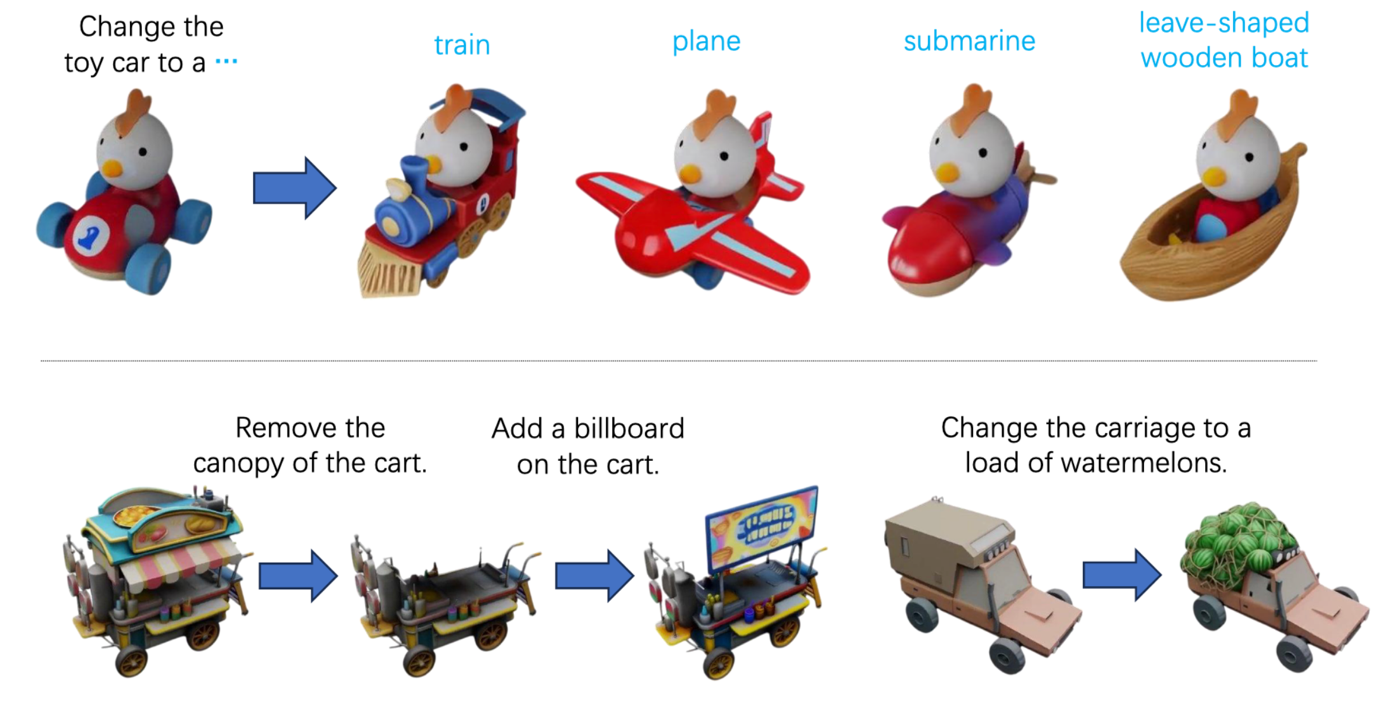
\includegraphics[width=0.90\linewidth]{asset_edit_examples.png}
  \caption{三维资产局部编辑示例：文本指令可对应颜色、部件、形状和物体级修改。}
  \label{fig:asset-edit}
\end{figure}

对于更复杂的结构级编辑，可以采用 Vinedresser3D 类局部编辑框架：先由多模态模型判断编辑意图和目标部件，再在结构化三维 latent 中进行局部 inpainting，最后将结果转换回可渲染资产。该思路适合处理“给模型加上某个部件”“改变某个局部形状”这类单纯高斯平移难以完成的任务。

\begin{figure}[H]
  \centering
  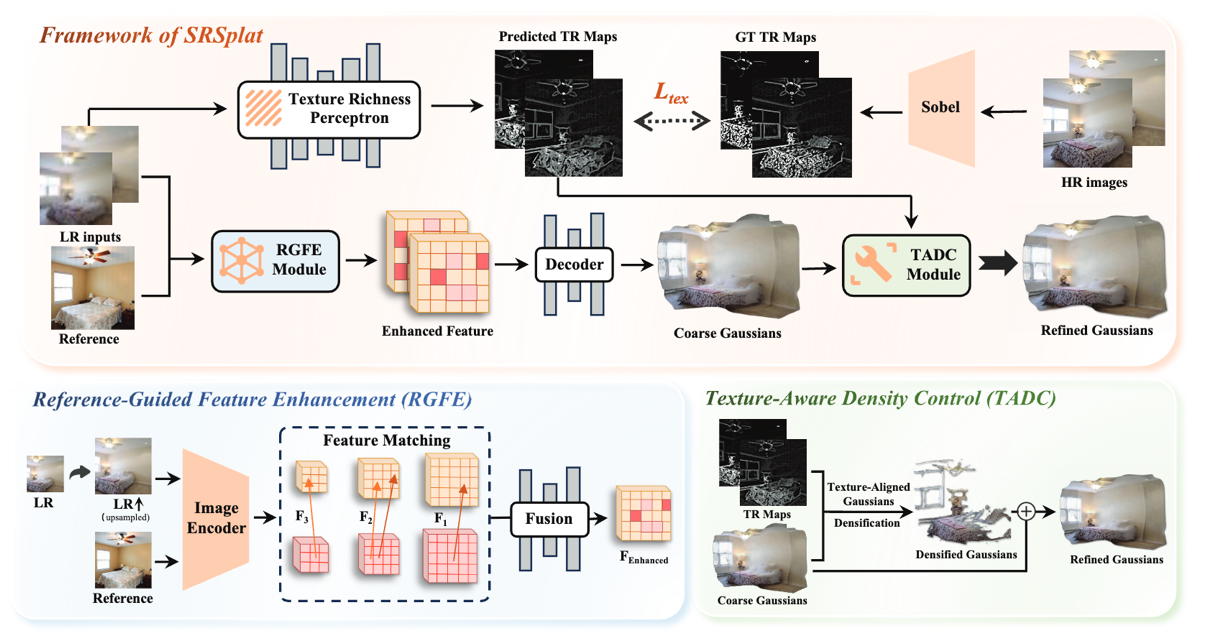
\includegraphics[width=0.95\linewidth]{vinedresser_framework.png}
  \caption{面向三维资产局部精修的编辑框架示意：语言理解、区域定位和局部生成共同完成结构级编辑。}
  \label{fig:vinedresser}
\end{figure}

实验分析表明，3DGS 的显式表示让几何操作更直接：删除目标对象相当于移除一组高斯，平移或缩放相当于修改高斯中心和协方差；但语义级编辑的核心困难在于“选中正确的高斯”。若二维分割 mask 不稳定，或者目标在不同视角下被遮挡，三维聚合得到的 $\mathcal{G}_{target}$ 就会混入背景高斯，导致编辑边界发虚或误删。因此，多视角一致性约束和可保护区域建模是编辑模块的关键。

本实验将编辑任务拆分为“可直接参数操作”和“需要生成补全”两类。删除、移动、缩放、复制和简单变色属于前者，主要依赖三维 mask 质量；替换物体、增加新物体、改变形状结构属于后者，需要 Trellis、Vinedresser3D 或类似生成模型提供目标资产。对于校园场景，前者适合快速清理重建结果中的漂浮物或不需要的局部对象，后者适合插入虚拟讲解牌、课程展示模型、AR 导览元素等内容。

\subsection{方法对比与课程理解}

表 \ref{tab:method-comparison} 对比了本实验涉及的主要技术。可以看到，VGGT 更适合作为快速几何前端，3DGS 更适合作为高质量可编辑表示，而语言驱动三维编辑方法负责把用户意图转换为具体高斯操作。三者组合后，能够形成比单一模型更完整的系统能力。

\begin{table}[H]
  \centering
  \caption{相关方法在本实验中的作用对比}
  \label{tab:method-comparison}
  \begin{tabularx}{\linewidth}{p{2.5cm} p{3.1cm} p{3.1cm} X}
    \toprule
    \textbf{方法} & \textbf{优势} & \textbf{局限} & \textbf{在本实验中的作用} \\
    \midrule
    SfM/MVS & 几何解释清晰，工程成熟 & 弱纹理和动态场景下容易失败 & 可作为相机估计和点云初始化基线 \\
    VGGT & 前馈预测相机、深度、点图，速度快 & 结果仍受训练分布和输入质量影响 & 为 3DGS 提供更稳健的几何先验 \\
    NeRF & 连续隐式表示，视图合成质量高 & 训练/渲染较慢，局部编辑不直观 & 提供神经渲染背景和对比参照 \\
    3DGS & 实时渲染，显式高斯可操作 & 弱纹理区域和动态物体仍困难 & 作为校园场景重建和编辑的核心表示 \\
    语言驱动编辑 & 降低三维编辑门槛 & 语义定位和边界保持仍有误差 & 将自然语言映射为三维局部操作 \\
    \bottomrule
  \end{tabularx}
\end{table}

从深度学习课程角度看，本实验体现了多种关键思想：Transformer 可用于跨视角几何推理；可微渲染将三维重建转化为端到端优化问题；显式参数化表示能提升可解释性与可编辑性；多模态大模型则把语言、图像和三维空间连接起来。相比只做分类或检测任务，三维重建与编辑更强调数据采集、几何约束、渲染模型和交互需求之间的系统协同。

\subsection{从单场景到可编辑三维内容系统}

如果把本实验进一步扩展为完整系统，还需要考虑场景组合与资产管理问题。LiSee 项目中提到的图文双驱路线并不只是“重建一个场景”或“生成一个物体”，而是要把真实场景、生成资产、编辑指令和导出格式组织成统一工作流。SynCity 等工作说明，大语言模型可以先把复杂场景描述拆成若干对象级或区域级子任务，再调用图像/三维生成模型生成局部内容，最后进行空间拼接和一致性校验。

\begin{figure}[H]
  \centering
  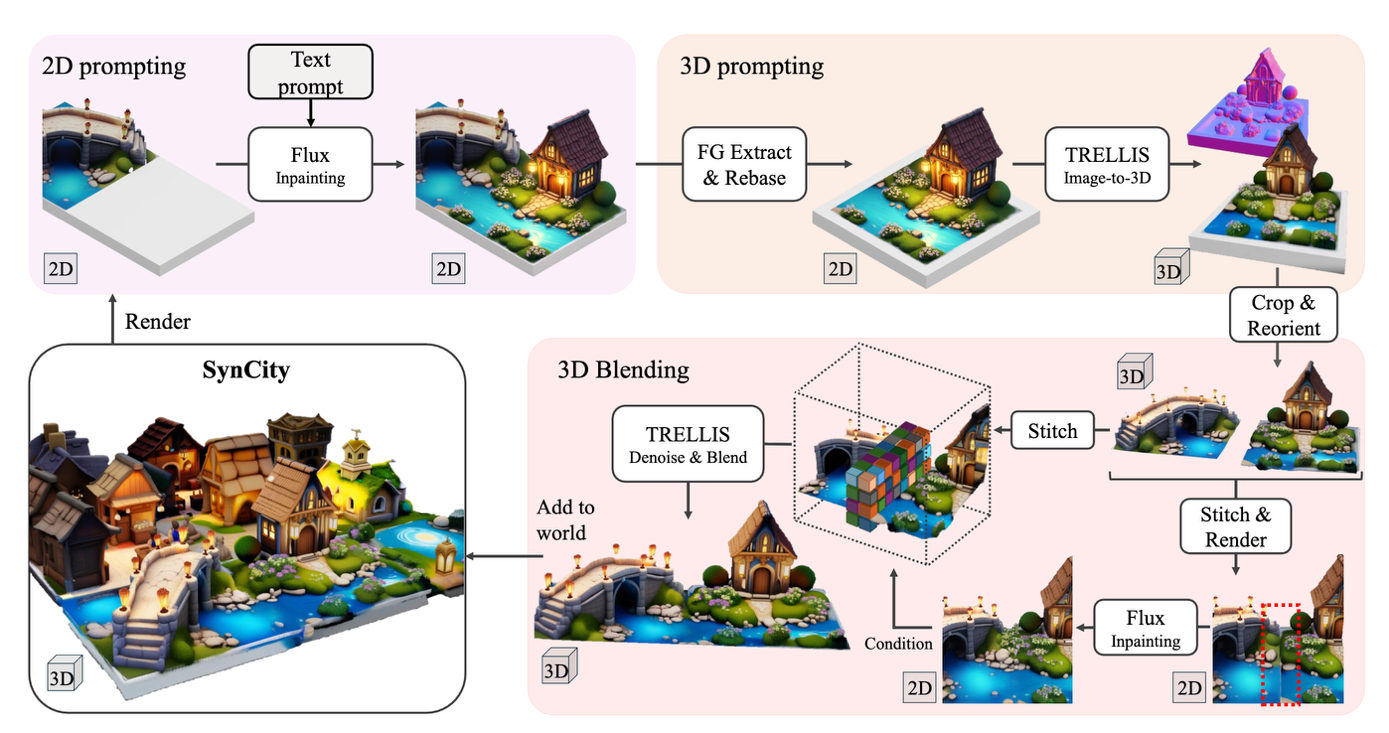
\includegraphics[width=0.95\linewidth]{syncity_pipeline.png}
  \caption{大场景生成中的语言规划和局部组合思想，可为校园数字孪生中的多区域编辑提供参考。}
  \label{fig:syncity}
\end{figure}

该思想可以迁移到校园重建中。例如，用户输入“在计算机学院门口生成一个课程展览区”，系统可以先将任务拆解为展板、桌台、讲解模型、路径标识等子对象；每个对象由生成模型产生三维资产，再通过尺度估计和地面支撑约束放入 3DGS 场景。最后，语言编辑模块继续允许用户说“把展板移到左边”“换成蓝色主题”“删除多余桌台”等。由此，VGGT+3DGS 解决真实环境获取，Trellis/SynCity 类生成方法解决新内容供给，REALM/GaussianEditor 类编辑方法解决自然交互，三者共同构成可编辑三维内容系统。

\section{实验总结}

本报告完成了一条面向校园场景的三维重建与编辑技术方案：先利用 VGGT 估计多视角几何与相机关系，再通过 3D Gaussian Splatting 优化高质量可实时渲染的三维场景，最后基于显式高斯表示设计语义定位和局部编辑流程。实验素材覆盖校门、计算机学院、教室和实验室等真实场景，说明该路线具备构建校园数字资产和交互式三维展示的可行性。

实验也暴露出若干限制。第一，重建结果强依赖拍摄质量，视频压缩、运动模糊和弱纹理区域会直接影响高斯稳定性。第二，3DGS 虽然便于编辑，但语义对象并不会天然对应一组干净高斯，仍需要多视角 grounding、分割和三维聚合。第三，生成资产插入真实场景时，尺度、光照、接触关系和遮挡关系都需要额外约束，否则会出现悬浮或视觉割裂。

后续工作可以从三个方向推进：一是建立更规范的校园多视角数据采集流程，增加关键点覆盖和近景细节；二是在 3DGS 中引入实例特征或语义特征，使重建阶段就具备对象级可编辑结构；三是结合 LiSee 项目的图文双驱思路，把文本生成三维资产、真实场景融合和自然语言编辑接入同一高斯空间，形成“拍照重建、说话生成、局部修改、实时预览”的完整三维内容创作系统。

\newpage
\section{参考文献}

\begin{enumerate}[label={[\arabic*]}, leftmargin=2.2em]
  \item Mildenhall B, Srinivasan P P, Tancik M, et al. \emph{NeRF: Representing Scenes as Neural Radiance Fields for View Synthesis}. ECCV, 2020. \url{https://www.matthewtancik.com/nerf}
  \item Kerbl B, Kopanas G, Leimkuehler T, Drettakis G. \emph{3D Gaussian Splatting for Real-Time Radiance Field Rendering}. ACM Transactions on Graphics, 2023. \url{https://repo-sam.inria.fr/fungraph/3d-gaussian-splatting/}
  \item Wang J, Karaev N, Rupprecht C, Novotny D. \emph{VGGT: Visual Geometry Grounded Transformer}. 2025. \url{https://vgg-t.github.io/}
  \item Haque A, Tancik M, Efros A A, Holynski A, Kanazawa A. \emph{Instruct-NeRF2NeRF: Editing 3D Scenes with Instructions}. ICCV, 2023. \url{https://instruct-nerf2nerf.github.io/}
  \item Chen Y, Chen Z, Zhang C, et al. \emph{GaussianEditor: Swift and Controllable 3D Editing with Gaussian Splatting}. CVPR, 2024. \url{https://buaacyw.github.io/gaussian-editor/}
  \item Shi C, Chen M, Mao Y, et al. \emph{REALM: An MLLM-Agent Framework for Open World 3D Reasoning Segmentation and Editing on Gaussian Splatting}. CVPR, 2026.
  \item Poole B, Jain A, Barron J T, Mildenhall B. \emph{DreamFusion: Text-to-3D using 2D Diffusion}. ICLR, 2023. \url{https://dreamfusion3d.github.io/}
  \item Xiang J, Lv Z, Xu S, et al. \emph{Structured 3D Latents for Scalable and Versatile 3D Generation}. 2024. \url{https://trellis3d.github.io/}
  \item Chi Y, Li X, Huang Z, et al. \emph{Vinedresser3D: Agentic Text-guided 3D Editing}. 2026.
  \item Engstler P, Shtedritski A, Laina I, et al. \emph{SynCity: Training-Free Generation of 3D Worlds}. 2025.
\end{enumerate}

\end{document}
